\documentclass[aspectratio=169]{beamer}
\usepackage{tikz}
\usetikzlibrary{arrows.meta, positioning, shapes.geometric, fit, backgrounds, calc}
\beamertemplatenavigationsymbolsempty
\setbeamertemplate{frametitle}{}
\setbeamercolor{background canvas}{bg=white}

\tikzset{
    flowbase/.style={node distance=0.25cm and 0.2cm, font=\tiny, >={Stealth[length=2pt]}},
    process/.style={rectangle, draw, rounded corners=2pt, fill=blue!8, minimum height=0.38cm, text width=2.1cm, align=center, inner sep=1pt},
    crypto/.style={rectangle, draw, rounded corners=2pt, fill=orange!15, minimum height=0.38cm, text width=2.1cm, align=center, inner sep=1pt},
    decision/.style={diamond, draw, fill=yellow!15, minimum height=0.3cm, inner sep=0.5pt, aspect=2.2, align=center},
    data/.style={rectangle, draw, fill=green!10, minimum height=0.35cm, text width=2.0cm, align=center, inner sep=1pt},
    startstop/.style={rectangle, draw, rounded corners=5pt, fill=gray!15, minimum height=0.35cm, align=center, inner sep=1.5pt},
    flowlabel/.style={font=\tiny\itshape, text=black!70},
    line/.style={draw, ->, thick, color=black!70},
}

\begin{document}

% ================================================================
%  SLIDE 1: Bidder Registration + Auction Creation
% ================================================================
\begin{frame}[t]
\vspace{-2mm}
\begin{center}
{\Large\bfseries Sealed-Bid Auction System --- Setup Phase}
\end{center}
\vspace{-2mm}

\begin{tikzpicture}[flowbase]

% ===================== COLUMN 1: BIDDER REGISTRATION =====================
\node[startstop] (r_start) at (0, 0) {Bidder Registration};
\node[process, below=of r_start] (r_id) {Enter Bidder ID \& Name};
\node[decision, below=of r_id] (r_dup) {ID exists?};
\node[process, below left=0.25cm and 0.1cm of r_dup] (r_reject) {Reject};
\node[process, below=0.4cm of r_dup] (r_pw) {Enter Password\\(8+ chars, upper,\\digit, symbol)};
\node[crypto, below=of r_pw] (r_keygen) {Generate ECDSA\\key pair (P-256)};
\node[crypto, below=of r_keygen] (r_enc) {Encrypt priv key\\scrypt($N\!=\!2^{17}$, r=8, p=1)\\+ ChaCha20-Poly1305};
\node[data, below=of r_enc] (r_store) {Store: pub.pem,\\priv.enc.json,\\profile.json};
\node[data, below=of r_store] (r_fp) {Compute key fingerprint\\SHA-256 of DER pubkey\\(first 8 bytes as XX:XX)};

\draw[line] (r_start) -- (r_id);
\draw[line] (r_id) -- (r_dup);
\draw[line] (r_dup) -- node[left, flowlabel]{yes} (r_reject);
\draw[line] (r_dup) -- node[right, flowlabel]{no} (r_pw);
\draw[line] (r_pw) -- (r_keygen);
\draw[line] (r_keygen) -- (r_enc);
\draw[line] (r_enc) -- (r_store);
\draw[line] (r_store) -- (r_fp);

% ===================== COLUMN 2: AUCTION CREATION =====================
\node[startstop] (a_start) at (5.5, 0) {Auction Creation};
\node[process, below=of a_start] (a_name) {Set auction name,\\deadline, bid limits\\(min/max optional)};
\node[process, below=of a_name] (a_tn) {Set threshold\\$t$-of-$n$ authorities\\($t \geq 2$, $n \geq 2$)};
\node[process, below=of a_tn] (a_auth_loop) {For each authority $i$:\\set ID \& password};
\node[crypto, below=of a_auth_loop] (a_keygen) {Generate ECDSA\\key pair per authority\\(P-256)};
\node[crypto, below=of a_keygen] (a_enc_auth) {Encrypt each priv key\\scrypt($N\!=\!2^{20}$, r=8, p=1)\\+ ChaCha20-Poly1305};
\node[crypto, below=of a_enc_auth] (a_hash) {SHA-256 hash of\\meta.json (canonical JSON:\\sorted keys, no spaces)};
\node[data, below=of a_hash] (a_ledger) {Ledger: append\\AUCTION\_CREATED\\with meta\_hash};
\node[data, below=of a_ledger] (a_meta) {Save meta.json:\\deadline, $t$, $n$,\\authority pubkeys,\\crypto parameters};

\draw[line] (a_start) -- (a_name);
\draw[line] (a_name) -- (a_tn);
\draw[line] (a_tn) -- (a_auth_loop);
\draw[line] (a_auth_loop) -- (a_keygen);
\draw[line] (a_keygen) -- (a_enc_auth);
\draw[line] (a_enc_auth) -- (a_hash);
\draw[line] (a_hash) -- (a_ledger);
\draw[line] (a_ledger) -- (a_meta);

% ===================== LEGEND =====================
\node[anchor=north west] at (9.5, 0) {%
\begin{tikzpicture}[font=\tiny, node distance=0.25cm]
    \node[font=\scriptsize\bfseries] (leg_title) {Legend};
    \node[rectangle, draw, rounded corners=2pt, fill=blue!8, minimum height=0.3cm, text width=1.8cm, align=center, below=0.15cm of leg_title] (l1) {User input / logic};
    \node[rectangle, draw, rounded corners=2pt, fill=orange!15, minimum height=0.3cm, text width=1.8cm, align=center, below=0.1cm of l1] (l2) {Crypto operation};
    \node[rectangle, draw, fill=green!10, minimum height=0.3cm, text width=1.8cm, align=center, below=0.1cm of l2] (l3) {Data / output};
    \node[diamond, draw, fill=yellow!15, minimum height=0.2cm, inner sep=0.5pt, aspect=2.2, align=center, below=0.1cm of l3] (l4) {Decision};
    \node[rectangle, draw, rounded corners=5pt, fill=gray!15, minimum height=0.3cm, text width=1.8cm, align=center, below=0.1cm of l4] (l5) {Workflow start};
\end{tikzpicture}};

% ===================== STORAGE LAYOUT NOTE =====================
\node[anchor=north west, text width=3.5cm, font=\tiny] at (9.5, -4) {%
\textbf{On-disk layout (store/):}\\[1pt]
\texttt{auctions/\{id\}/meta.json}\\
\texttt{auctions/\{id\}/ledger.log}\\
\texttt{auctions/\{id\}/bids/*.json}\\
\texttt{auctions/\{id\}/authorities/}\\
\texttt{~~\{auth\_id\}/pub.pem}\\
\texttt{~~\{auth\_id\}/priv.enc.json}\\
\texttt{users/bidders/\{id\}/pub.pem}\\
\texttt{users/bidders/\{id\}/priv.enc.json}\\
\texttt{users/bidders/\{id\}/profile.json}
};

% ===================== DEADLINE FORMATS NOTE =====================
\node[anchor=north west, text width=3.5cm, font=\tiny] at (9.5, -2.2) {%
\textbf{Deadline formats accepted:}\\[1pt]
\texttt{2026-03-15 14:30:00} (LK)\\
\texttt{2026-03-15T09:00:00Z} (UTC)\\
\texttt{in 30 min / in 2 hours}\\[1pt]
Stored as UTC with Z suffix.\\
Display: Asia/Colombo (UTC+05:30)
};

\end{tikzpicture}
\end{frame}

% ================================================================
%  SLIDE 2: Bid Submission + Reveal & Winner
% ================================================================
\begin{frame}[t]
\vspace{-2mm}
\begin{center}
{\Large\bfseries Sealed-Bid Auction System --- Bidding \& Reveal Phase}
\end{center}
\vspace{-2mm}

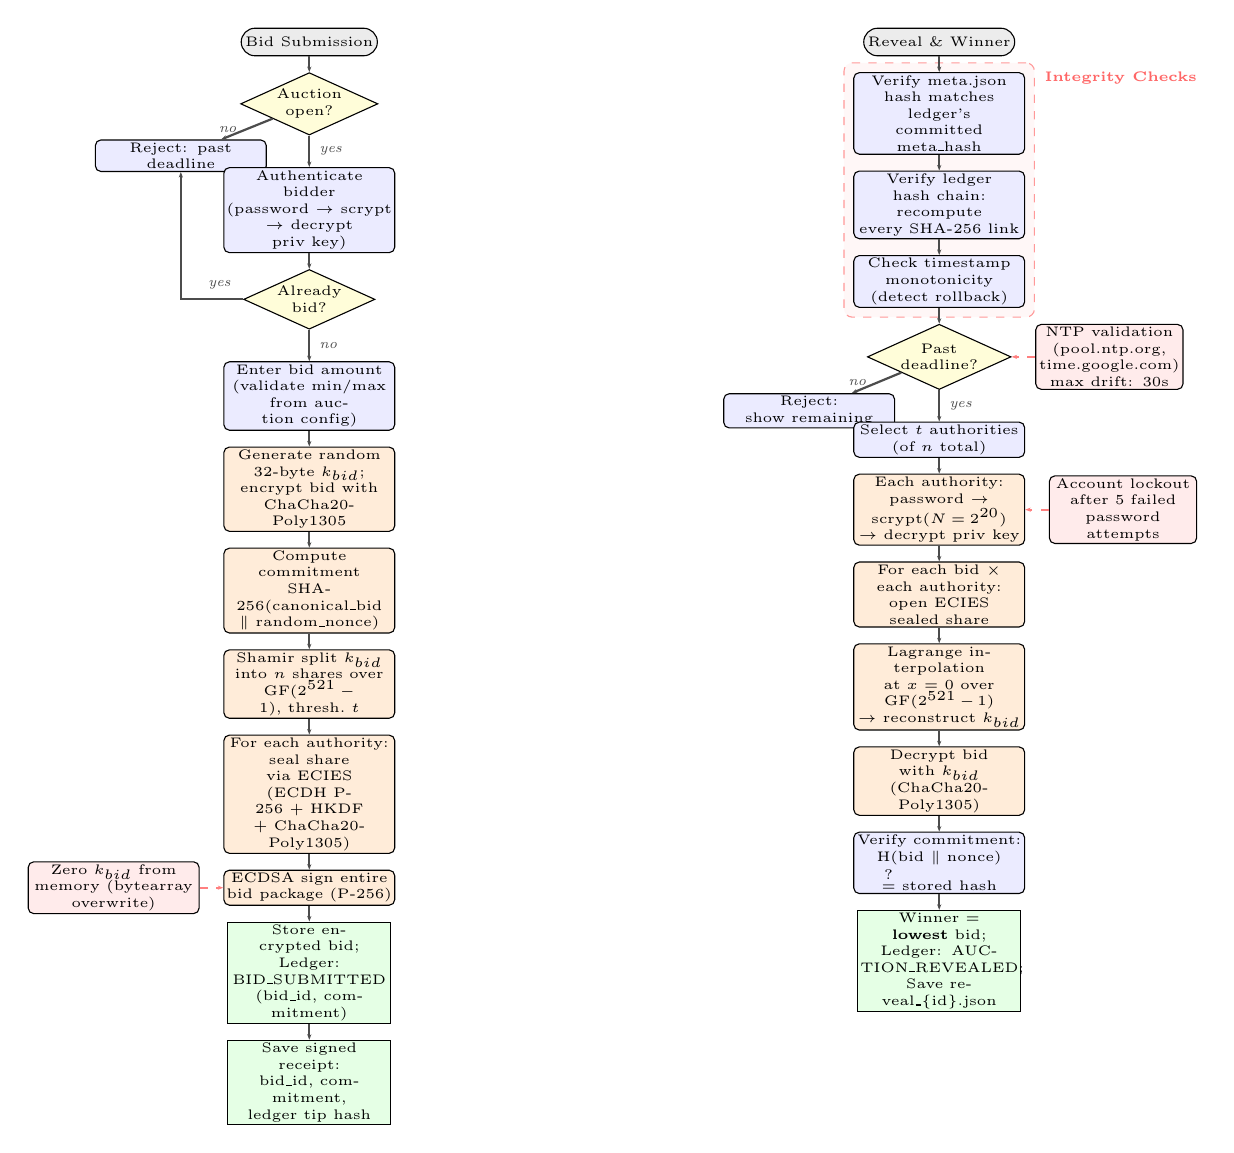
\begin{tikzpicture}[flowbase, node distance=0.2cm and 0.15cm]

% ===================== COLUMN 1: BID SUBMISSION =====================
\node[startstop] (b_start) at (0, 0) {Bid Submission};
\node[decision, below=of b_start] (b_state) {Auction\\open?};
\node[process, below left=0.25cm and 0.1cm of b_state] (b_closed) {Reject: past\\deadline};
\node[process, below=0.4cm of b_state] (b_auth) {Authenticate bidder\\(password $\to$ scrypt\\$\to$ decrypt priv key)};
\node[decision, below=of b_auth] (b_dup) {Already\\bid?};
\node[process, below=0.4cm of b_dup] (b_amount) {Enter bid amount\\(validate min/max\\from auction config)};
\node[crypto, below=of b_amount] (b_enc) {Generate random\\32-byte $k_{bid}$;\\encrypt bid with\\ChaCha20-Poly1305};
\node[crypto, below=of b_enc] (b_commit) {Compute commitment\\SHA-256(canonical\_bid\\$\|$ random\_nonce)};
\node[crypto, below=of b_commit] (b_shamir) {Shamir split $k_{bid}$\\into $n$ shares over\\GF($2^{521}\!-\!1$), thresh.~$t$};
\node[crypto, below=of b_shamir] (b_seal) {For each authority:\\seal share via ECIES\\(ECDH P-256 + HKDF\\+ ChaCha20-Poly1305)};
\node[crypto, below=of b_seal] (b_sign) {ECDSA sign entire\\bid package (P-256)};

\draw[line] (b_start) -- (b_state);
\draw[line] (b_state) -- node[left, flowlabel]{no} (b_closed);
\draw[line] (b_state) -- node[right, flowlabel]{yes} (b_auth);
\draw[line] (b_auth) -- (b_dup);
\draw[line] (b_dup.west) -- ++(-0.3,0) node[above, flowlabel]{yes} -| (b_closed);
\draw[line] (b_dup) -- node[right, flowlabel]{no} (b_amount);
\draw[line] (b_amount) -- (b_enc);
\draw[line] (b_enc) -- (b_commit);
\draw[line] (b_commit) -- (b_shamir);
\draw[line] (b_shamir) -- (b_seal);
\draw[line] (b_seal) -- (b_sign);

% Storage + ledger for bid
\node[data, below=of b_sign] (b_store) {Store encrypted bid;\\Ledger: BID\_SUBMITTED\\(bid\_id, commitment)};
\node[data, below=of b_store] (b_receipt) {Save signed receipt:\\bid\_id, commitment,\\ledger tip hash};
\draw[line] (b_sign) -- (b_store);
\draw[line] (b_store) -- (b_receipt);

% Zero key note
\node[process, fill=red!8, left=0.3cm of b_sign] (b_zero) {Zero $k_{bid}$ from\\memory (bytearray\\overwrite)};
\draw[->, dashed, red!50, thick] (b_zero) -- (b_sign);

% ===================== COLUMN 2: REVEAL & WINNER =====================
\node[startstop] (v_start) at (8, 0) {Reveal \& Winner};
\node[process, below=of v_start] (v_meta) {Verify meta.json\\hash matches ledger's\\committed meta\_hash};
\node[process, below=of v_meta] (v_ledger) {Verify ledger\\hash chain: recompute\\every SHA-256 link};
\node[process, below=of v_ledger] (v_ts) {Check timestamp\\monotonicity\\(detect rollback)};
\node[decision, below=of v_ts] (v_deadline) {Past\\deadline?};
\node[process, below left=0.25cm and 0.1cm of v_deadline] (v_wait) {Reject:\\show remaining};
\node[process, below=0.4cm of v_deadline] (v_select) {Select $t$ authorities\\(of $n$ total)};
\node[crypto, below=of v_select] (v_unlock) {Each authority:\\password $\to$ scrypt($N\!=\!2^{20}$)\\$\to$ decrypt priv key};
\node[crypto, below=of v_unlock] (v_unseal) {For each bid $\times$\\each authority:\\open ECIES sealed share};
\node[crypto, below=of v_unseal] (v_recon) {Lagrange interpolation\\at $x\!=\!0$ over GF($2^{521}\!-\!1$)\\$\to$ reconstruct $k_{bid}$};
\node[crypto, below=of v_recon] (v_dec) {Decrypt bid with $k_{bid}$\\(ChaCha20-Poly1305)};
\node[process, below=of v_dec] (v_verify) {Verify commitment:\\H(bid $\|$ nonce)\\$\stackrel{?}{=}$ stored hash};
\node[data, below=of v_verify] (v_winner) {Winner = \textbf{lowest} bid;\\Ledger: AUCTION\_REVEALED;\\Save reveal\_\{id\}.json};

\draw[line] (v_start) -- (v_meta);
\draw[line] (v_meta) -- (v_ledger);
\draw[line] (v_ledger) -- (v_ts);
\draw[line] (v_ts) -- (v_deadline);
\draw[line] (v_deadline) -- node[left, flowlabel]{no} (v_wait);
\draw[line] (v_deadline) -- node[right, flowlabel]{yes} (v_select);
\draw[line] (v_select) -- (v_unlock);
\draw[line] (v_unlock) -- (v_unseal);
\draw[line] (v_unseal) -- (v_recon);
\draw[line] (v_recon) -- (v_dec);
\draw[line] (v_dec) -- (v_verify);
\draw[line] (v_verify) -- (v_winner);

% ===================== SECURITY ANNOTATIONS =====================
% NTP annotation
\node[process, fill=red!8, text width=1.8cm, right=0.3cm of v_deadline] (v_ntp) {NTP validation\\(pool.ntp.org,\\time.google.com)\\max drift: 30s};
\draw[->, dashed, red!50, thick] (v_ntp) -- (v_deadline);

% Account lockout annotation
\node[process, fill=red!8, text width=1.8cm, right=0.3cm of v_unlock] (v_lock) {Account lockout\\after 5 failed\\password attempts};
\draw[->, dashed, red!50, thick] (v_lock) -- (v_unlock);

% Integrity checks background
\begin{scope}[on background layer]
    \node[draw=red!40, dashed, fill=red!3, rounded corners=3pt,
          fit=(v_meta)(v_ledger)(v_ts),
          label={[font=\tiny\bfseries, text=red!60]above right:Integrity Checks}] {};
\end{scope}

\end{tikzpicture}
\end{frame}

\end{document}
